\documentclass{standalone}

\usepackage{tikz}
\usepackage{xcolor}
\usepackage{amsmath}
\usepackage{nicefrac}

\definecolor{jet}{HTML}{363636}
\definecolor{outerspace}{HTML}{464646}
\definecolor{granitegray}{HTML}{616161}
\definecolor{raisinblack}{HTML}{252525}
\definecolor{tigerseye}{HTML}{EB9438}
\definecolor{denimblue}{HTML}{2B3EAB}
\definecolor{englishgreen}{HTML}{26523C}
\definecolor{upmaroon}{HTML}{780D14}
\definecolor{isabelline}{HTML}{EDEDED}
\definecolor{palmleaf}{HTML}{6DA63F}

\usetikzlibrary{shapes.arrows,chains}
\newcommand{\I}{\color{isabelline}}
\newcommand{\N}{{\color{tigerseye} n}\I}

\begin{document}

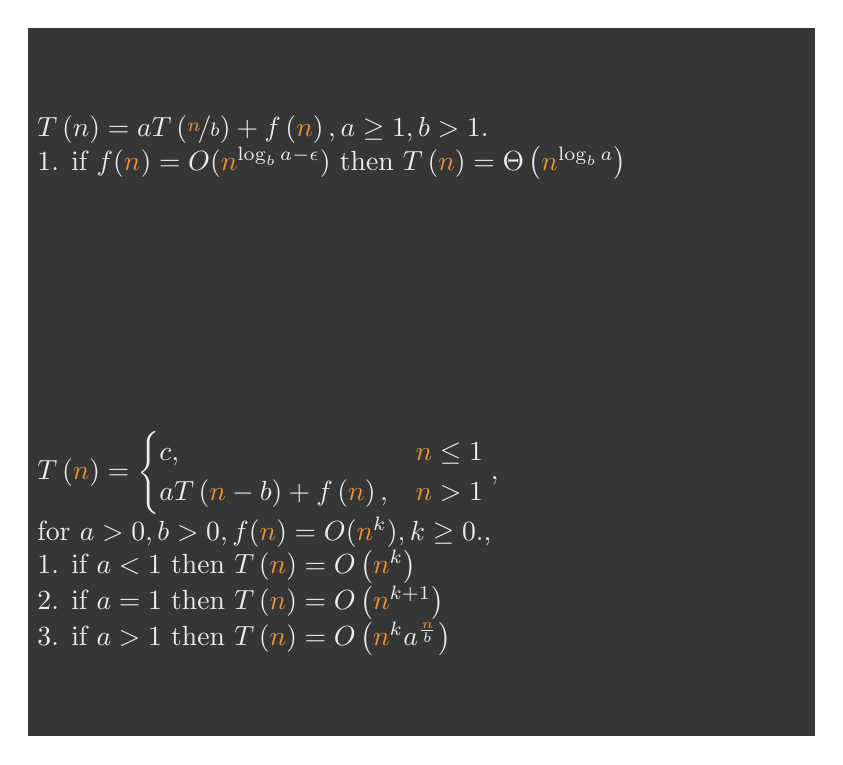
\begin{tikzpicture}
  % Background
  \fill [jet] (0, -4) rectangle (10, 5);

  \node[align=left] at(0, 4)[anchor=north west] {
    $\I T\left(n\right)=aT\left(\nicefrac{\N}{b}\right) + f\left(\N\right), a \ge 1, b > 1.$\\
    \I 1. if $f(\N)=O(\N^{\log_{b} a - \epsilon})$ then $T\left(\N\right) = \Theta\left(\N^{\log_{b} a}\right)$
  };
  \node[align=left] at(0, 0)[anchor=north west] {
    $\I T\left(\N \right)=
        \begin{cases}
          c,& \N \le 1 \\
          aT\left(\N - b\right) + f\left(\N\right),& \N > 1
        \end{cases},$\\
     \I for $a > 0, b > 0, f(\N) = O(\N^{k}), k \ge 0.$,\\
     \I 1. if $a<1$ then $T\left(\N\right) = O\left(\N^{k}\right)$\\
     \I 2. if $a=1$ then $T\left(\N\right) = O\left(\N^{k + 1}\right)$\\
     \I 3. if $a>1$ then $T\left(\N\right) = O\left(\N^{k}a^{\frac{\N}{b}}\right)$
  };
\end{tikzpicture}

\end{document}
